\documentclass[xcolor=dvipsnames]{beamer}
\usepackage[T1]{fontenc}
\usepackage[utf8]{inputenc}
\usepackage[english,slovak]{babel}

\usepackage{amsmath}
\usepackage{amsthm}
\usetheme{Pittsburgh}
\useoutertheme{shadow}

\usepackage{amsmath}
\usepackage{amscd,amssymb,amsfonts}


\usepackage{graphicx}
\usepackage{caption}
\usepackage{subcaption}
\usepackage{listings}

\iffalse
%\iftrue
\usetheme{Warsaw}
% \usecolortheme{beetle}

\setbeamercolor{normal text}{fg=white,bg=black!90}
\setbeamercolor{structure}{fg=white}

\setbeamercolor{alerted text}{fg=red!85!black}

\setbeamercolor{item projected}{use=item,fg=black,bg=item.fg!35}

\setbeamercolor*{palette primary}{use=structure,fg=structure.fg}
\setbeamercolor*{palette secondary}{use=structure,fg=structure.fg!95!black}
\setbeamercolor*{palette tertiary}{use=structure,fg=structure.fg!90!black}
\setbeamercolor*{palette quaternary}{use=structure,fg=structure.fg!95!black,bg=black!80}

\setbeamercolor*{framesubtitle}{fg=white}

\setbeamercolor*{block title}{parent=structure,bg=black!60}
\setbeamercolor*{block body}{fg=black,bg=black!10}
\setbeamercolor*{block title alerted}{parent=alerted text,bg=black!15}
\setbeamercolor*{block title example}{parent=example text,bg=black!15}
\fi


\lstset{language=C++,
                basicstyle=\ttfamily,
                keywordstyle=\color{blue}\ttfamily,
                stringstyle=\color{red}\ttfamily,
                numberstyle=\color{green}\ttfamily,
                commentstyle=\color{green}\ttfamily,
                morecomment=[l][\color{magenta}]{\#}}

%-------------------------------------------------------------------------------------
\title{\bf Aproximácia funkcie ohodnotení v algoritmoch Q-learning neurónovou sieťou}
\author{Michal CHOVANEC \\Fakulta riadenia a informatiky}

\date[EURP]{\it Október 2015}
\begin{document}

\begin{frame}
\titlepage
školiteľ : prof. Ing. Juraj Miček, PhD. \\
rok štúdia : 3. \\
nástup na študium : 1.9.2013 \\
\end{frame}

%-------------------------------------------------------------------------------------
\begin{frame}{\bf Úvod}

Cieľom je nájsť optimálnu stratégiu - maximalizácia odmeny (účelovej funckie)

\begin{itemize}
\item{Vopred nie je známa hodnota odmeny vykonanej akcie}
\item{Vopred nie je známi ani stav do ktorého sa systém dostane}
\item{Je možné určiť v akom stave sa systém nachádza}
\item{Je presne daná množina akcií v každom stave}
\item{Aspoň pre cieľový stav je daná výška odmeny}
\end{itemize}

\end{frame}

%-------------------------------------------------------------------------------------
\begin{frame}{\bf Q learning - prechod stavovým priestorom}

%Markovov rozhodovací proces

\begin{figure}[ht]
\begin{center}
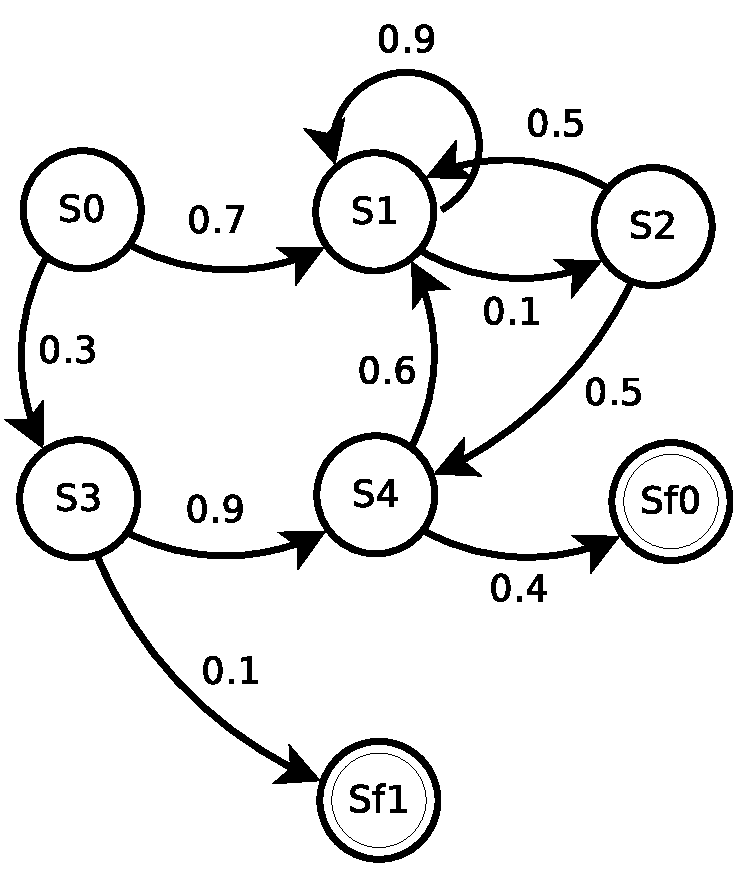
\includegraphics[width=0.5\textwidth]{diagrams/markov_decision.eps}
\end{center}
\end{figure}

\end{frame}

%-------------------------------------------------------------------------------------
\begin{frame}{\bf Q learning - ohodnotenie Q(s, a)}

\begin{equation}
\label{q_learning}
   Q_{n+1}(s, a) = R_{n+1}(s, a) + \gamma \max_{a'} Q_n(s_{n+1}', a')
\end{equation}

Kde \\
$R_{n+1}(s, a)$ je získaná odmena (reward) za vykonanie akcie $a$ v stave $s$ v čase
$n+1$ \\
\bigskip
$\max_{a'} Q_n(s_{n+1}', a')$ je výber akcie v stave $s_{n+1}$ ktorá má najväčšiu odmenu \\
\bigskip
$\gamma$ je podiel z maximálnej odmeny v stave $s_{n+1}'$ pri vykonaní najlepšej
možnej akcie v tomto stave

\end{frame}


%-------------------------------------------------------------------------------------
\begin{frame}{\bf Q learning - ohodnotenie Q(s, a)}

Varianty algoritmu \\

Filtrovanie v stochastickom prostredí
\begin{equation}
\label{q_learning}
   Q_{n+1}(s, a) = \alpha Q_{n}(s, a) + (1-\alpha) ( R_{n+1}(s, a) + \gamma \max_{a'} Q_n(s_{n+1}', a') ) \nonumber
\end{equation}

SARSA algoritmus
\begin{equation}
\label{q_learning}
   Q_{n+1}(s, a) = \alpha Q_{n}(s, a) + (1-\alpha) ( R_{n+1}(s, a) + \gamma Q_n(s_{n+1}', a') ) \nonumber
\end{equation}

\bigskip
kde $\alpha \in \langle 0, 1) $ \\

\end{frame}


%-------------------------------------------------------------------------------------
\begin{frame}{\bf Q learning - výber akcie}

Boltzmanové rozdelanie

\begin{equation}
P(s|a_i) = \frac{k^{Q(s, a_i)}} {{\sum_{j \in \mathbb{A}}{} k^{Q(s, a_j)}}} \nonumber
\end{equation}

Kde $k \in \langle 0, \infty )$ a určuje správanie sa agenta, pre $Q(s, a) \in \langle -1, 1 \rangle$
možno pozorovať tieto druhy správania

\begin{itemize}
\item{$k = 1$ prieskumník}
\item{$k = \langle 2, 10 \rangle$}
\item{$k >> 10$ pažravý (greedy) agent}
\end{itemize}

\end{frame}

%-------------------------------------------------------------------------------------
\begin{frame}{\bf Experiment}

Cieľom je overiť aproximáciu $Q(s, a)$ dvoma rôznymi neurónovými sieťami pri
rôznych veľkostiach $k$ v malom stavovom priestore - Q(s, a) vieme spočítať presne.

\begin{figure}[ht]
\begin{center}
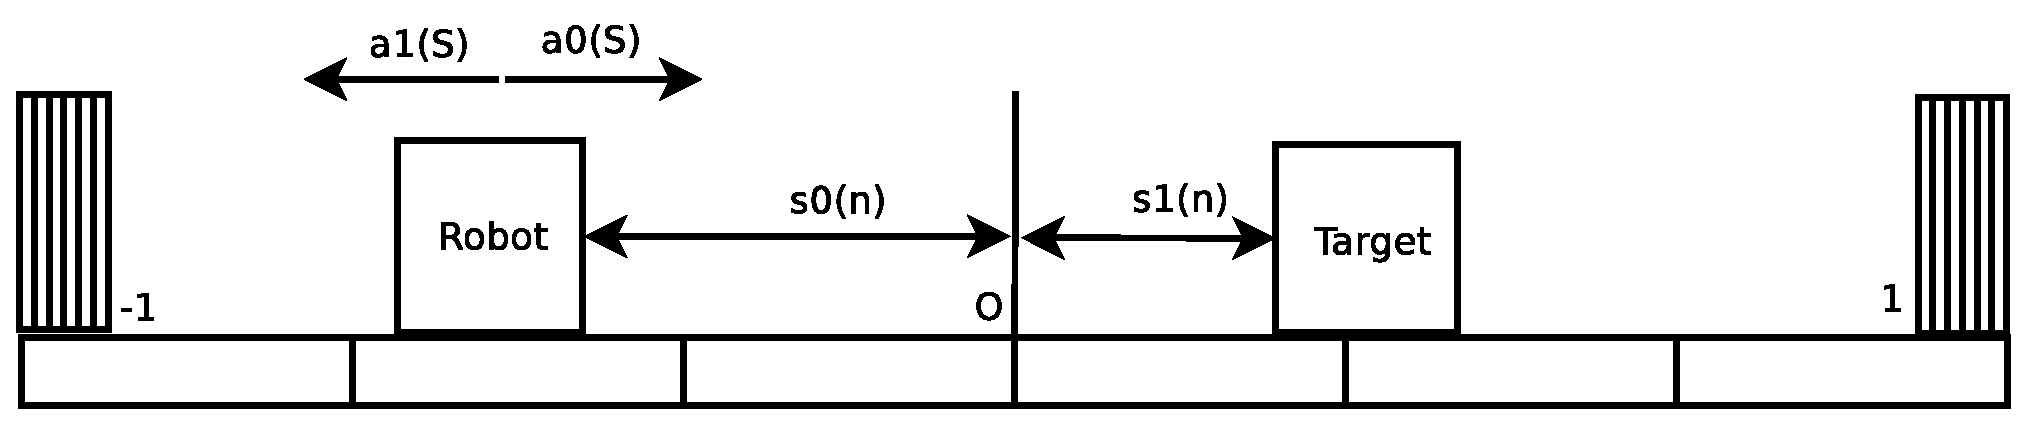
\includegraphics[width=0.8\textwidth]{diagrams/1D_robot_diagram.eps}
\end{center}
\end{figure}

\end{frame}

\iffalse

%-------------------------------------------------------------------------------------
\begin{frame}{\bf Experiment}

Boli porovnávané dva modely neurónov s optimálnym riešením

\begin{equation}
\label{mcculloch_pitts_model}
  y(n) = \varphi(\sum_{i = 0}^{N-1} x_i(n)w_i(n))
\end{equation}


\begin{equation}
\label{testing_neuron_model}
  y(n) = \sum_{j = 1}^{\infty}{\sum_{i = 0}^{N-1} x_i^j(n)w_{ji}(n)} +
  \sum_{j = 0}^{N-1}{\sum_{i = j + 1}^{N-1} x_i(n)x_j(n)v_{ji}(n)}
\end{equation}

Prečo by \ref{testing_neuron_model} mal byt lepší? Kolmogorov teorém 3 skryté vrstvy !

\end{frame}


%-------------------------------------------------------------------------------------
\begin{frame}{\bf Experiment}

Hypotéza : \\
\bigskip
Problém aproximácie $q = Q(s, a)$ je pridelenie každému $s$, $a$ práve jedno $q$.
To vedie na formuláciu : \\
AK je systém v stave s A bola vykonaná akcia a, POTOM výstup je q. \\
\bigskip
Pre jeden stav a dve akcie (ohodnotené ako $a_0$, $a_1$) možno napísať

\begin{equation}
\label{multiplexer}
  q =  v a_0 + (1 - v) a_1
\end{equation}

Kde $v$ je výber akcie a platí $v \in \langle 0, 1 \rangle$. Pozn. všetky veličiny
sú premenné.
\bigskip
To je ale potom v súlade s \ref{testing_neuron_model}.

\end{frame}

\fi

%-------------------------------------------------------------------------------------
\begin{frame}[fragile]{\bf Experiment - parametre}

\begin{lstlisting}

iterations = 10000000

agent :

state_density = 1/8.0
alpha = 0.98
gamma = 0.7

neural network :

hidden layers = 2
neurons in hidden layers = 10
weight range = 4.0
neuron order = 7
init weight range = 0.1
eta = 0.001

\end{lstlisting}

\end{frame}


%-------------------------------------------------------------------------------------
\begin{frame}{\bf Experiment, k = 1.1, optimálne riešenie}

\begin{columns}
	\begin{column}{0.5\textwidth}

        \begin{figure}[ht]

        \begin{center}
        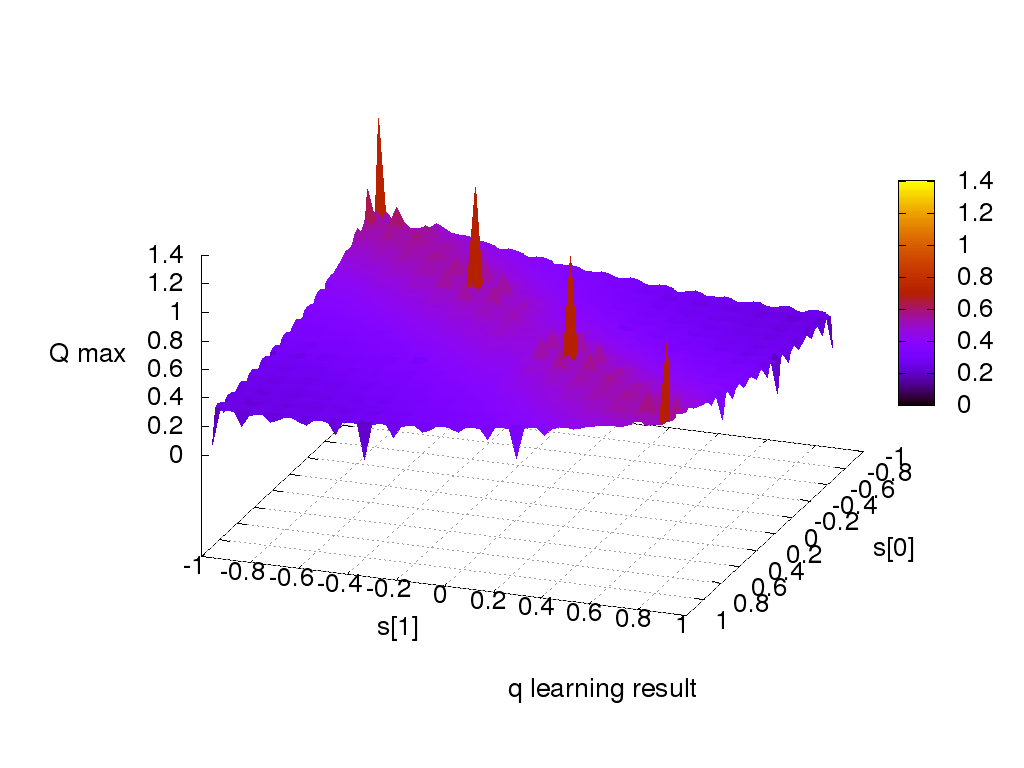
\includegraphics[width=1.0\textwidth]{experiment_01/table/q_map.png}
        \end{center}

        \end{figure}

	\end{column}
	\begin{column}{0.5\textwidth}

        \begin{figure}[ht]

        \begin{center}
        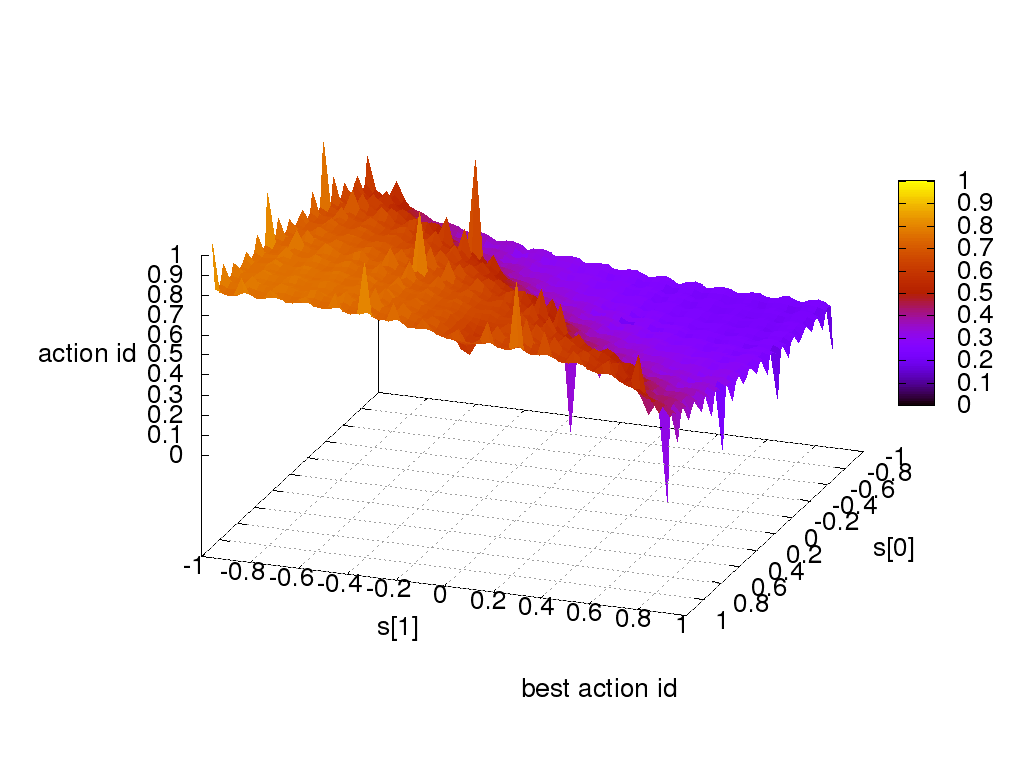
\includegraphics[width=1.0\textwidth]{experiment_01/table/q_action_id.png}
        \end{center}

        \end{figure}

	\end{column}
\end{columns}

\end{frame}


%-------------------------------------------------------------------------------------
\begin{frame}{\bf Experiment, k = 1.1, mcculloch pitts neurón}

\begin{columns}
	\begin{column}{0.5\textwidth}

        \begin{figure}[ht]

        \begin{center}
        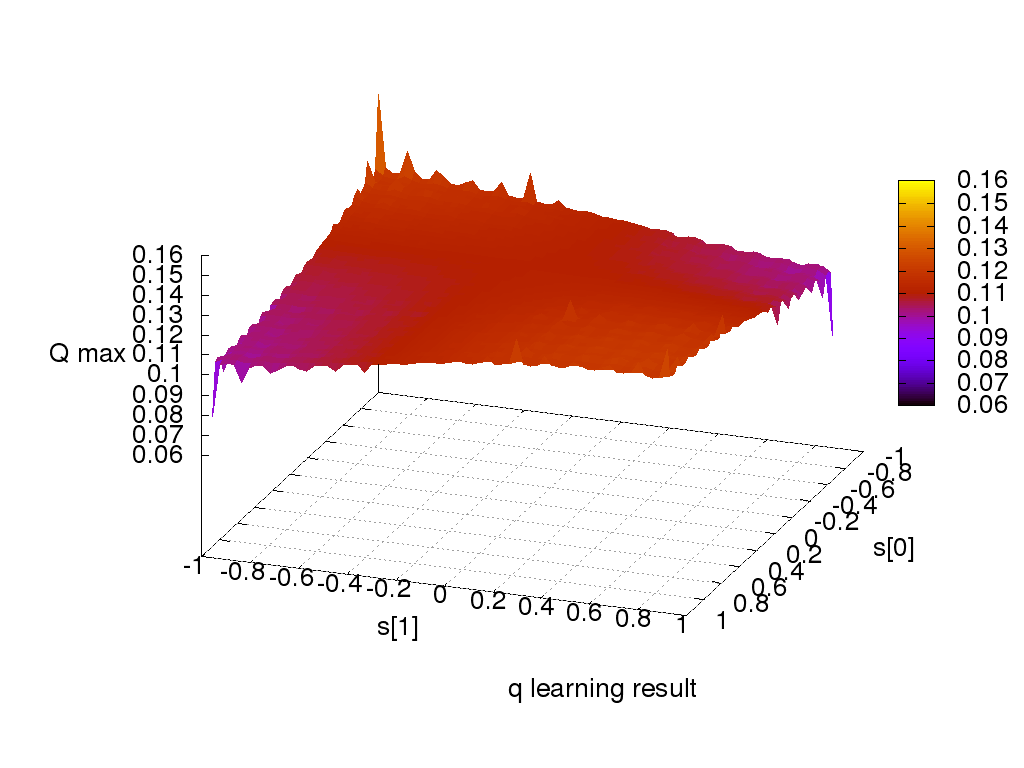
\includegraphics[width=1.0\textwidth]{experiment_01/mcculloch_pitts_neuron/q_map.png}
        \end{center}

        \end{figure}

	\end{column}
	\begin{column}{0.5\textwidth}

        \begin{figure}[ht]

        \begin{center}
        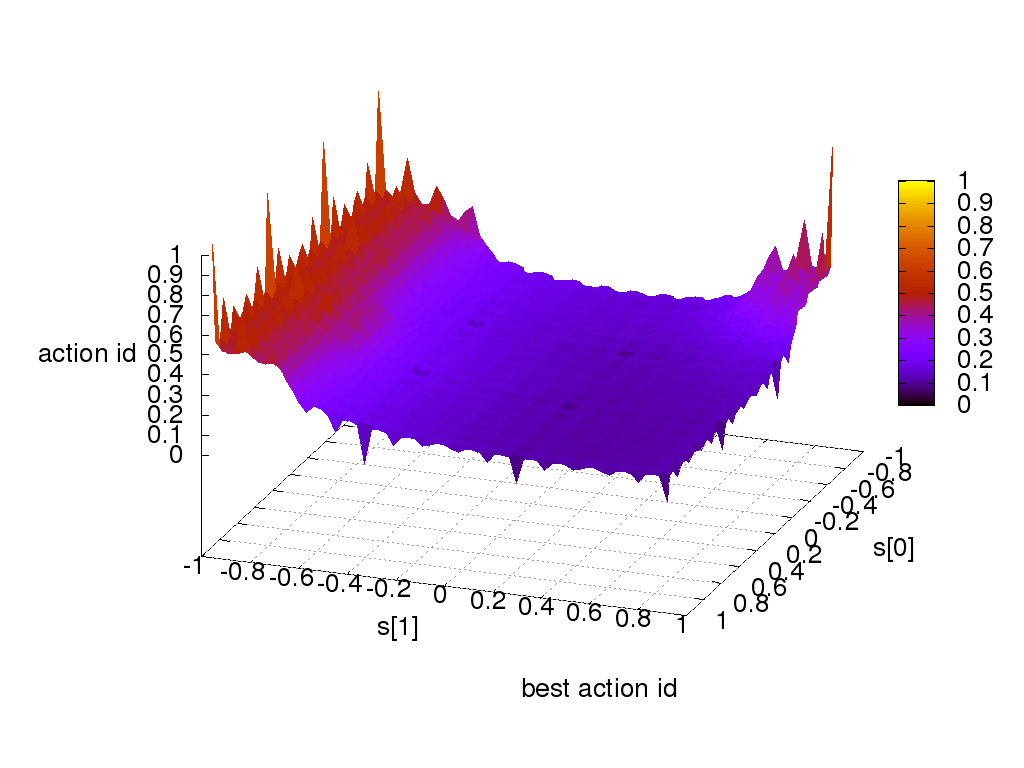
\includegraphics[width=1.0\textwidth]{experiment_01/mcculloch_pitts_neuron/q_action_id.png}
        \end{center}

        \end{figure}

	\end{column}
\end{columns}

\end{frame}


%-------------------------------------------------------------------------------------
\begin{frame}{\bf Experiment, k = 1.1, testovaný neurón}

\begin{columns}
	\begin{column}{0.5\textwidth}

        \begin{figure}[ht]

        \begin{center}
        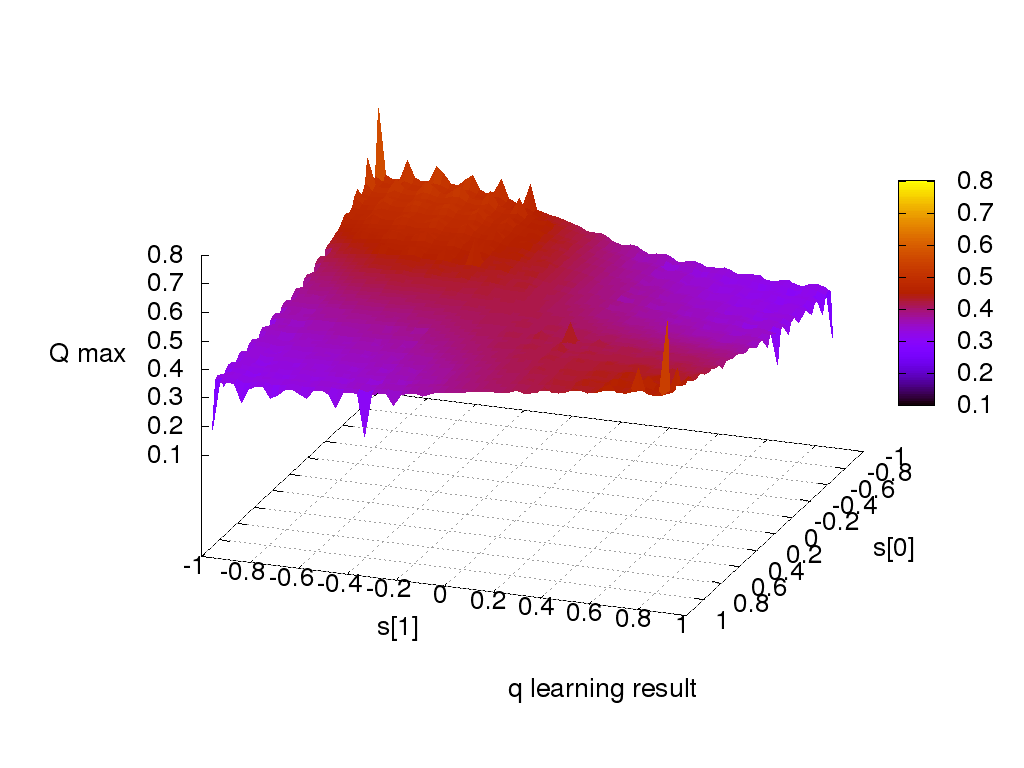
\includegraphics[width=1.0\textwidth]{experiment_01/testing_neuron/q_map.png}
        \end{center}

        \end{figure}

	\end{column}
	\begin{column}{0.5\textwidth}

        \begin{figure}[ht]

        \begin{center}
        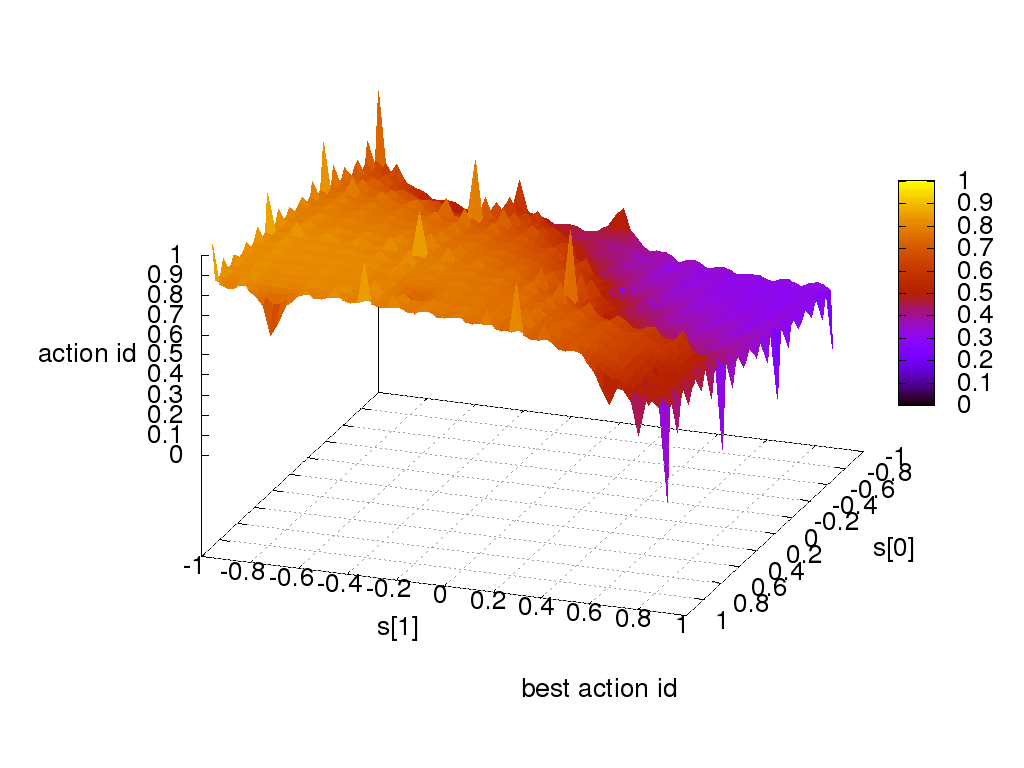
\includegraphics[width=1.0\textwidth]{experiment_01/testing_neuron/q_action_id.png}
        \end{center}

        \end{figure}

	\end{column}
\end{columns}

\end{frame}


%-------------------------------------------------------------------------------------
\begin{frame}{\bf Experiment, k = 2.0, optimálne riešenie}

\begin{columns}
	\begin{column}{0.5\textwidth}

        \begin{figure}[ht]

        \begin{center}
        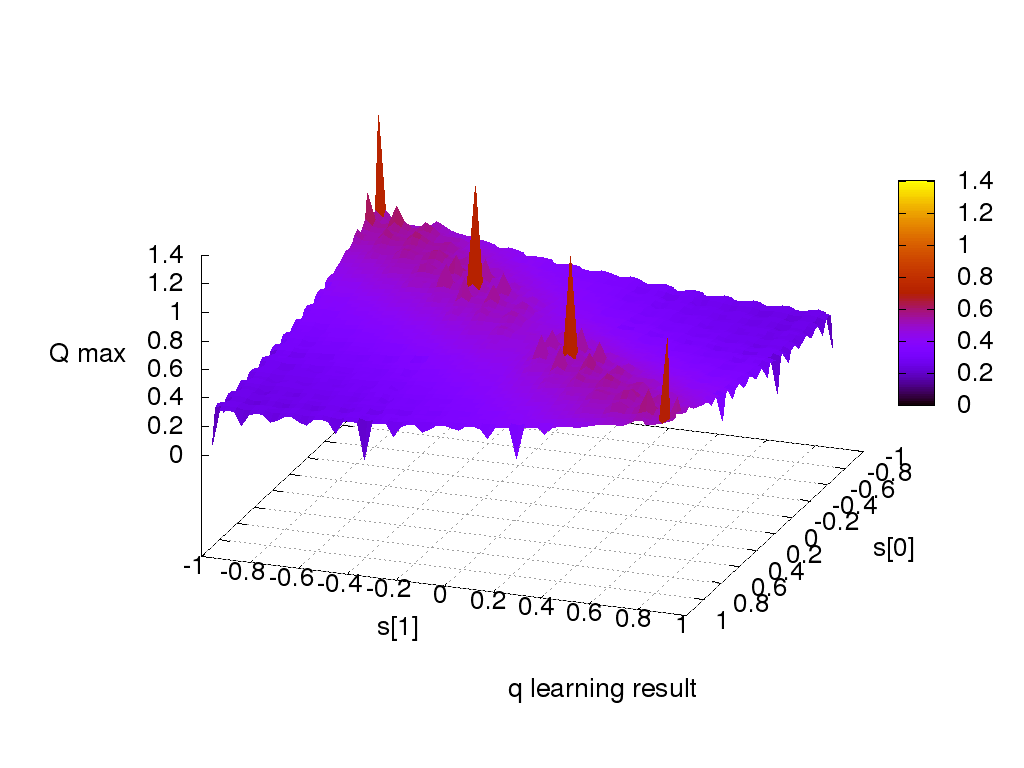
\includegraphics[width=1.0\textwidth]{experiment_02/table/q_map.png}
        \end{center}

        \end{figure}

	\end{column}
	\begin{column}{0.5\textwidth}

        \begin{figure}[ht]

        \begin{center}
        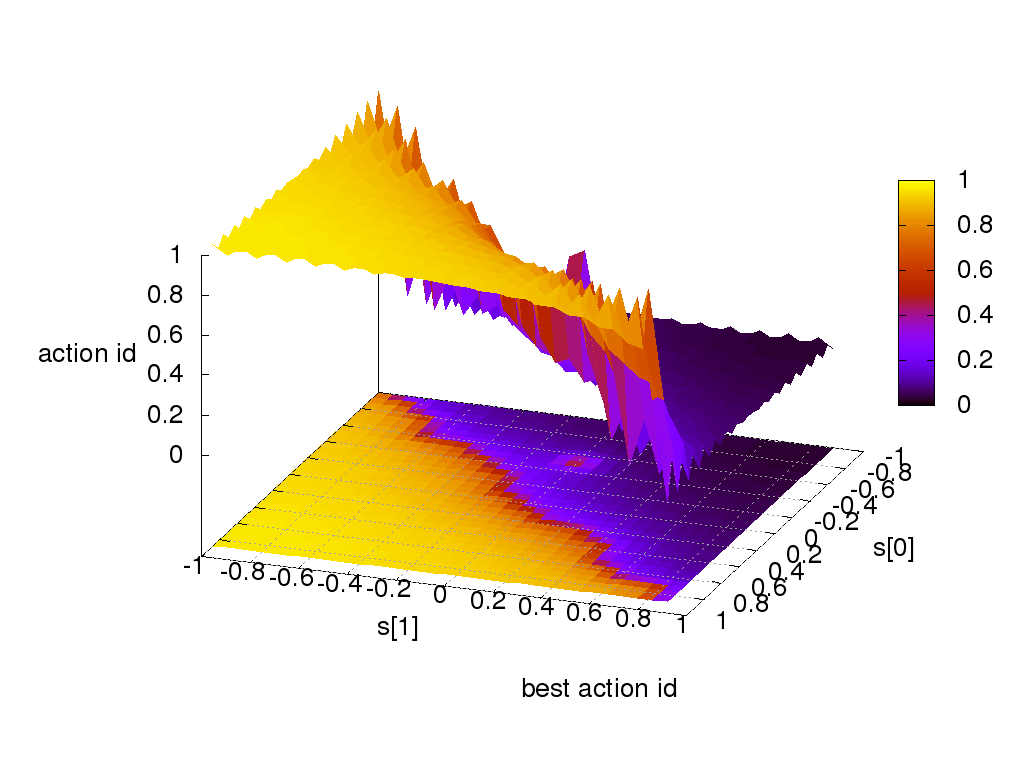
\includegraphics[width=1.0\textwidth]{experiment_02/table/q_action_id.png}
        \end{center}

        \end{figure}

	\end{column}
\end{columns}

\end{frame}


%-------------------------------------------------------------------------------------
\begin{frame}{\bf Experiment, k = 2.0, mcculloch pitts neurón}

\begin{columns}
	\begin{column}{0.5\textwidth}

        \begin{figure}[ht]

        \begin{center}
        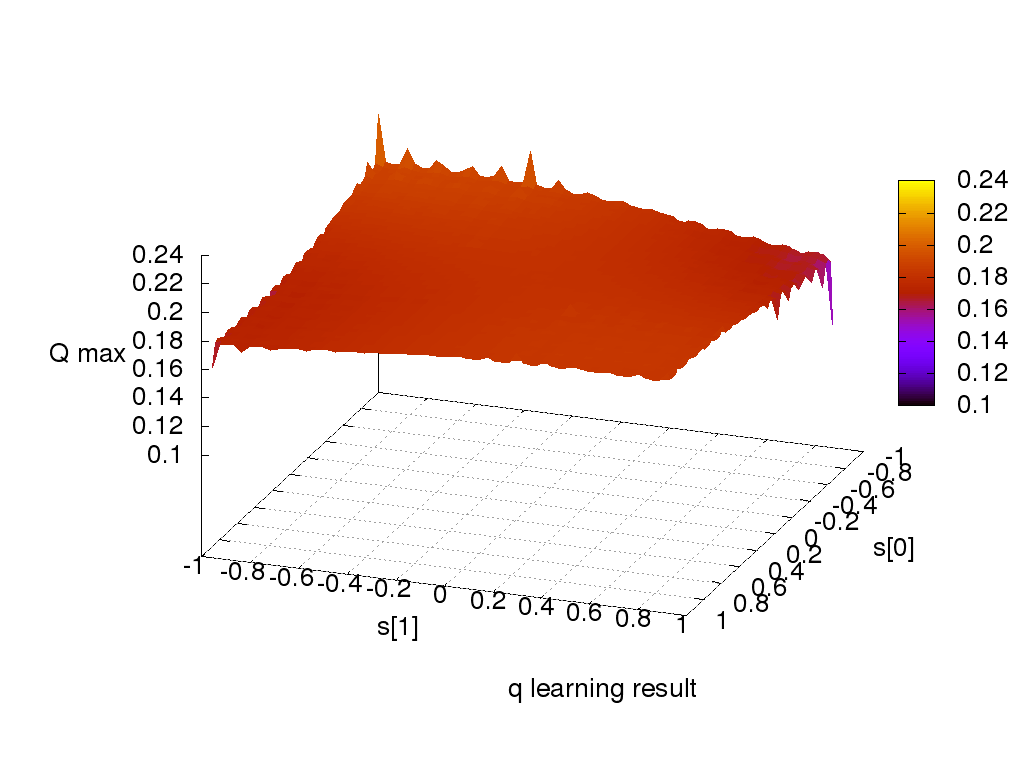
\includegraphics[width=1.0\textwidth]{experiment_02/mcculloch_pitts_neuron/q_map.png}
        \end{center}

        \end{figure}

	\end{column}
	\begin{column}{0.5\textwidth}

        \begin{figure}[ht]

        \begin{center}
        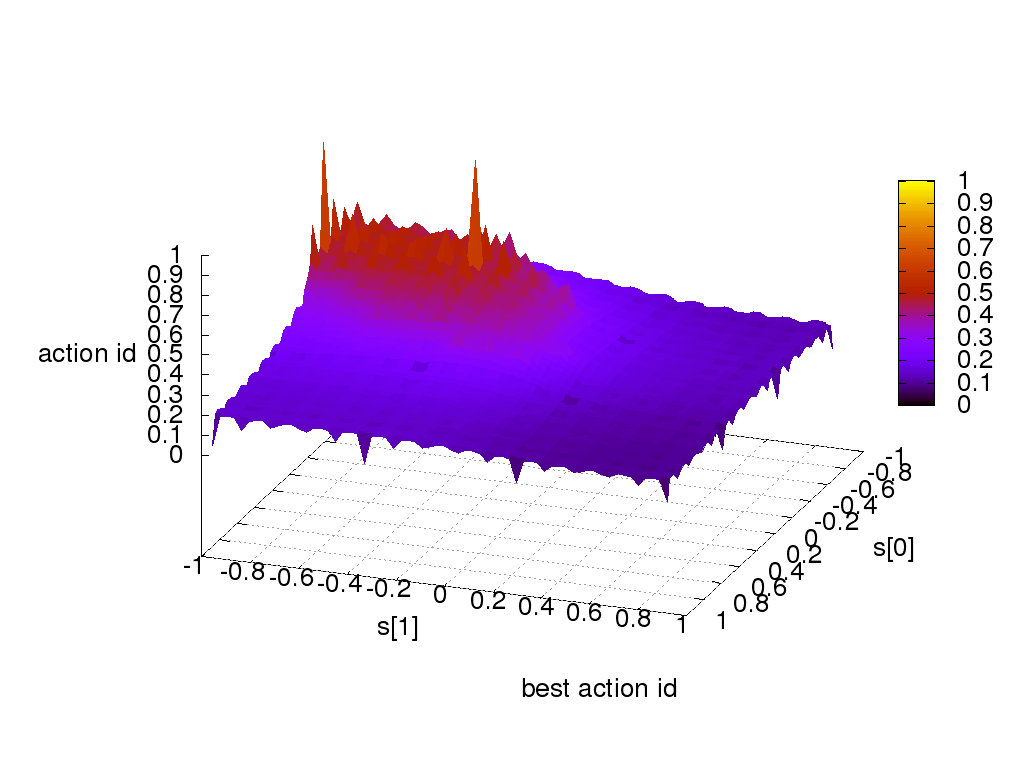
\includegraphics[width=1.0\textwidth]{experiment_02/mcculloch_pitts_neuron/q_action_id.png}
        \end{center}

        \end{figure}

	\end{column}
\end{columns}

\end{frame}


%-------------------------------------------------------------------------------------
\begin{frame}{\bf Experiment, k = 2.0, testovaný neurón}

\begin{columns}
	\begin{column}{0.5\textwidth}

        \begin{figure}[ht]

        \begin{center}
        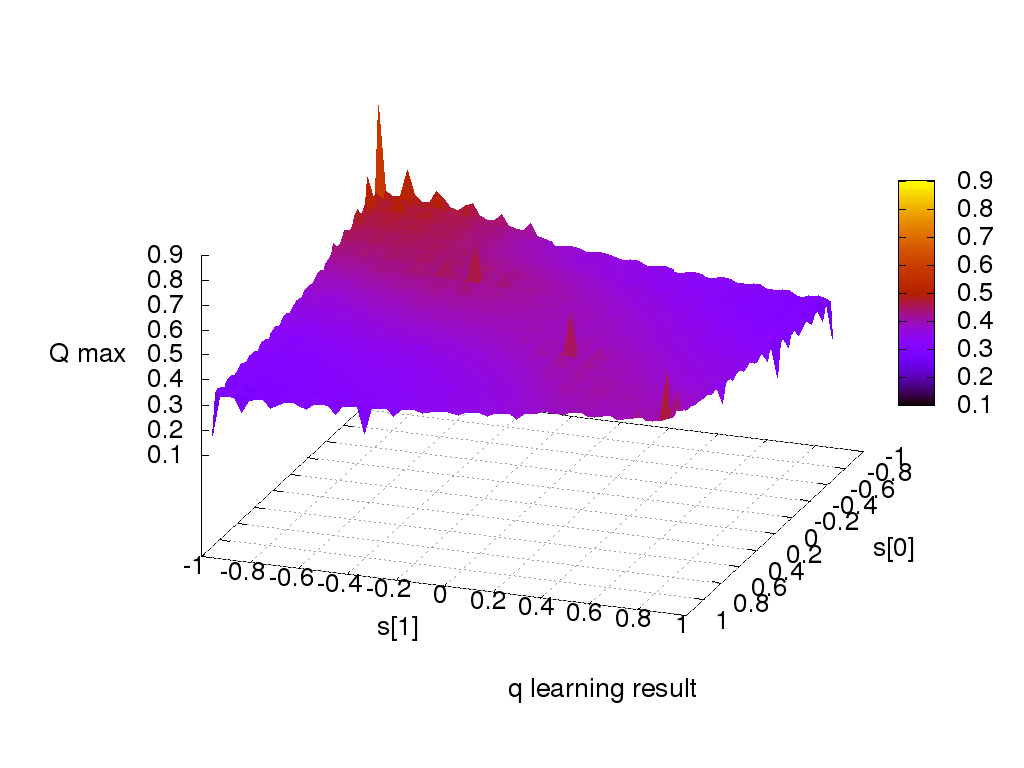
\includegraphics[width=1.0\textwidth]{experiment_02/testing_neuron/q_map.png}
        \end{center}

        \end{figure}

	\end{column}
	\begin{column}{0.5\textwidth}

        \begin{figure}[ht]

        \begin{center}
        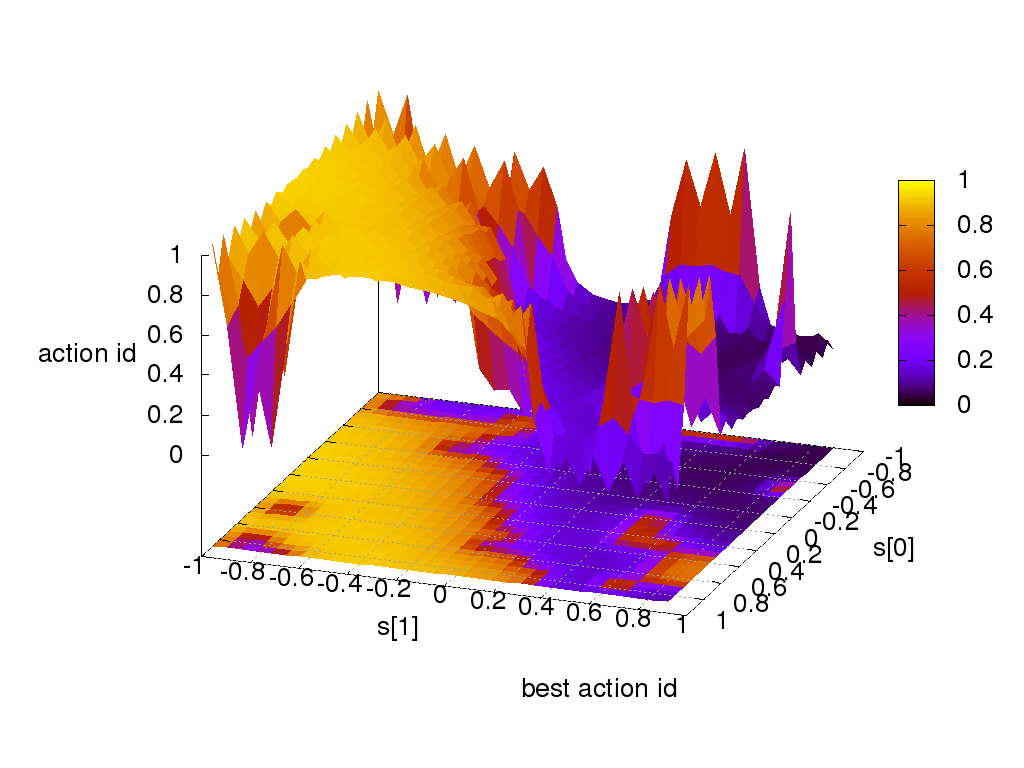
\includegraphics[width=1.0\textwidth]{experiment_02/testing_neuron/q_action_id.png}
        \end{center}

        \end{figure}

	\end{column}
\end{columns}

\end{frame}







%-------------------------------------------------------------------------------------
\begin{frame}{\bf Experiment, k = 10.0, optimálne riešenie}

\begin{columns}
	\begin{column}{0.5\textwidth}

        \begin{figure}[ht]

        \begin{center}
        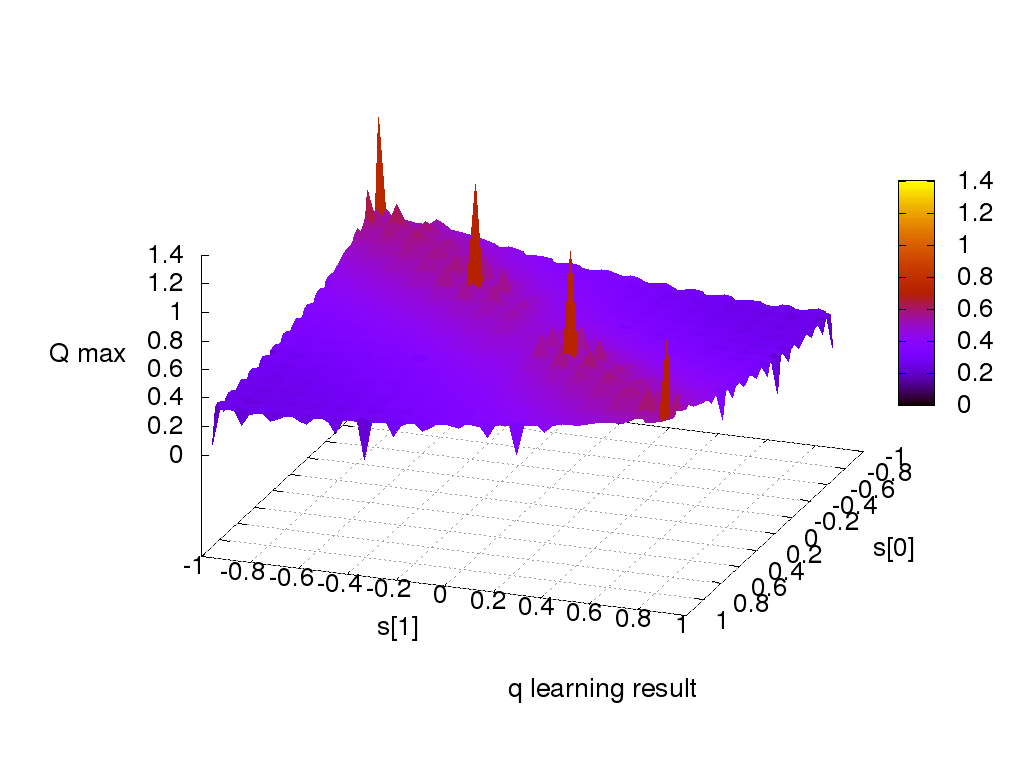
\includegraphics[width=1.0\textwidth]{experiment_03/table/q_map.png}
        \end{center}

        \end{figure}

	\end{column}
	\begin{column}{0.5\textwidth}

        \begin{figure}[ht]

        \begin{center}
        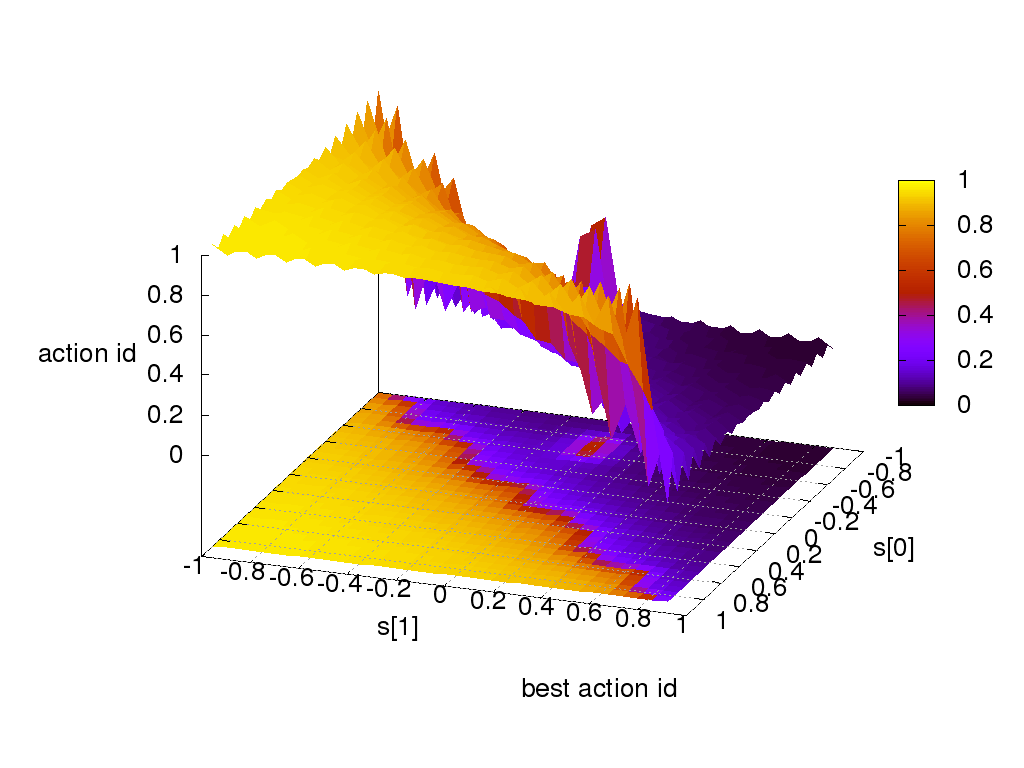
\includegraphics[width=1.0\textwidth]{experiment_03/table/q_action_id.png}
        \end{center}

        \end{figure}

	\end{column}
\end{columns}

\end{frame}


%-------------------------------------------------------------------------------------
\begin{frame}{\bf Experiment, k = 10.0, mcculloch pitts neurón}

\begin{columns}
	\begin{column}{0.5\textwidth}

        \begin{figure}[ht]

        \begin{center}
        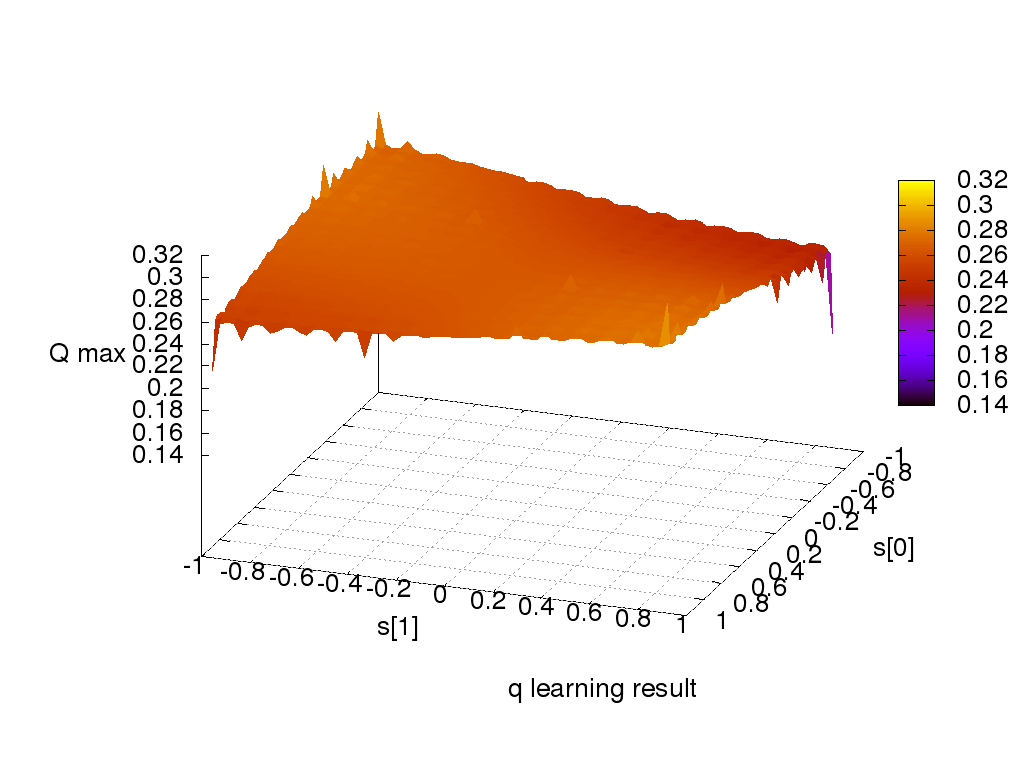
\includegraphics[width=1.0\textwidth]{experiment_03/mcculloch_pitts_neuron/q_map.png}
        \end{center}

        \end{figure}

	\end{column}
	\begin{column}{0.5\textwidth}

        \begin{figure}[ht]

        \begin{center}
        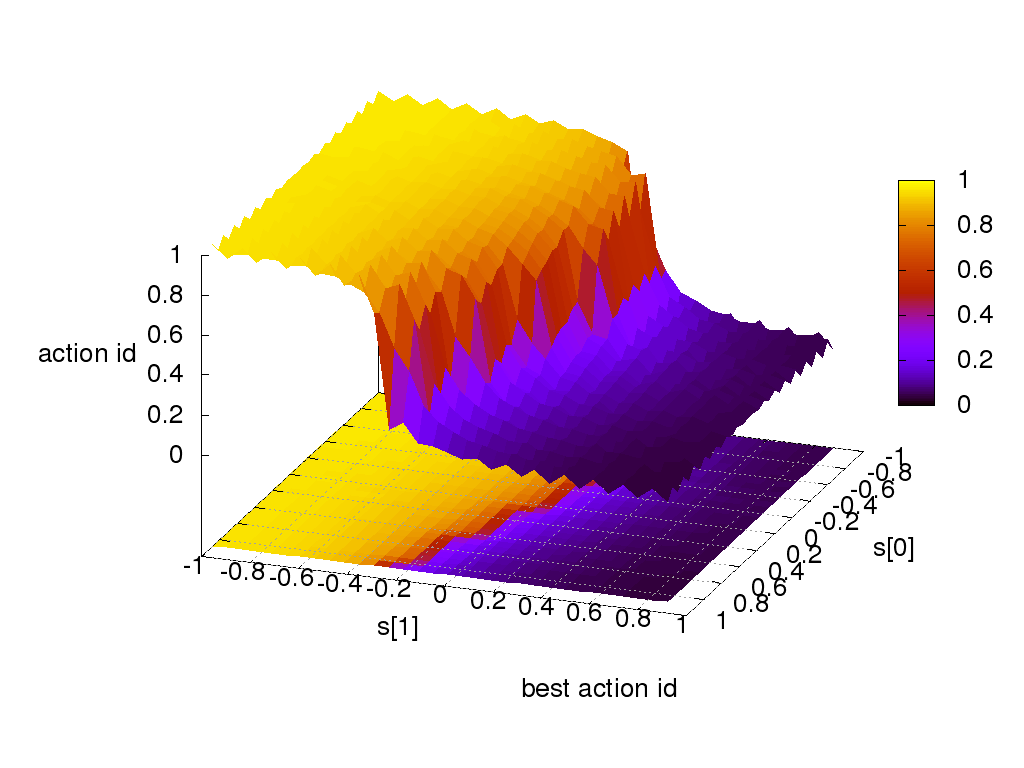
\includegraphics[width=1.0\textwidth]{experiment_03/mcculloch_pitts_neuron/q_action_id.png}
        \end{center}

        \end{figure}

	\end{column}
\end{columns}

\end{frame}


%-------------------------------------------------------------------------------------
\begin{frame}{\bf Experiment, k = 10.0, testovaný neurón}

\begin{columns}
	\begin{column}{0.5\textwidth}

        \begin{figure}[ht]

        \begin{center}
        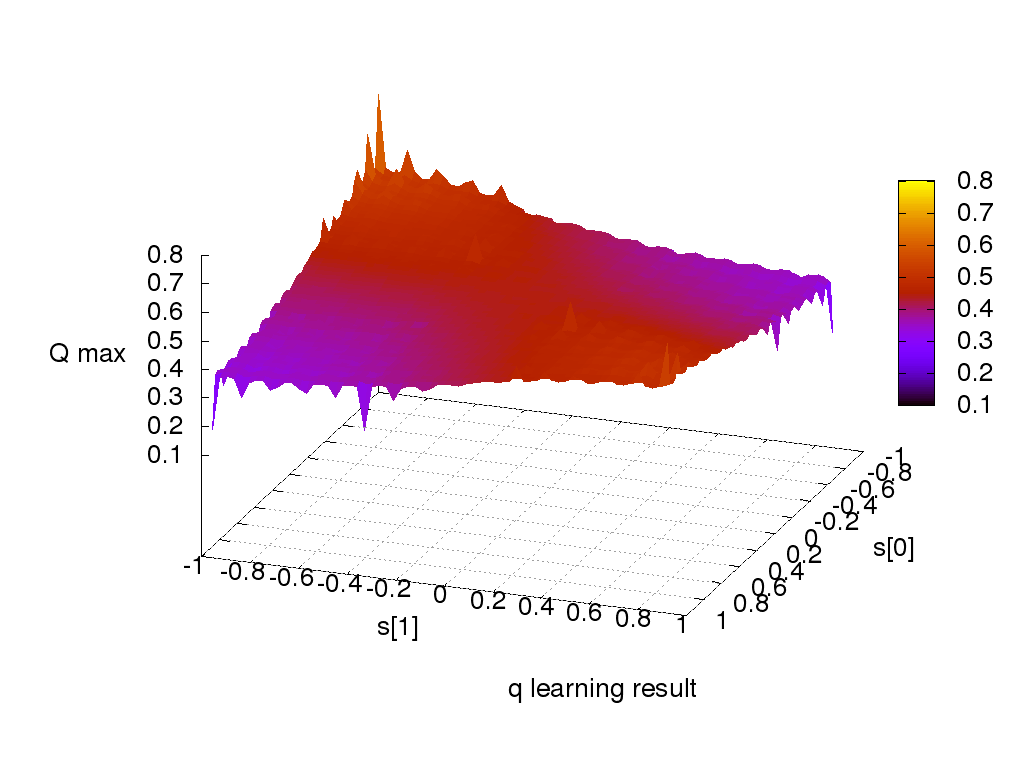
\includegraphics[width=1.0\textwidth]{experiment_03/testing_neuron/q_map.png}
        \end{center}

        \end{figure}

	\end{column}
	\begin{column}{0.5\textwidth}

        \begin{figure}[ht]

        \begin{center}
        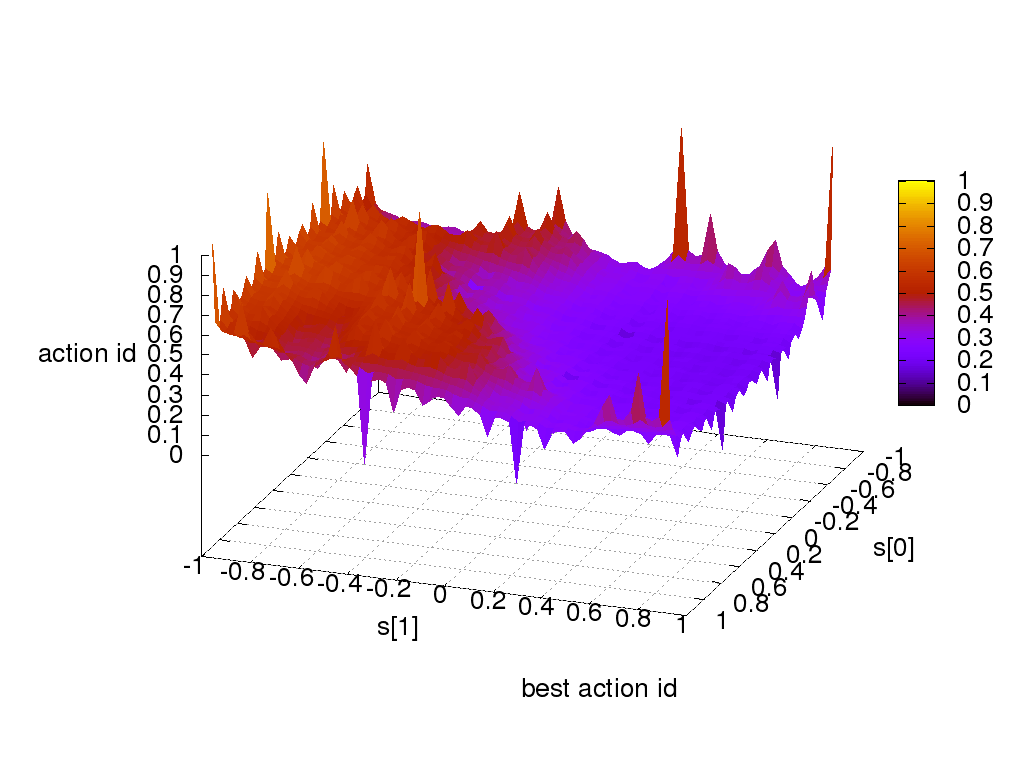
\includegraphics[width=1.0\textwidth]{experiment_03/testing_neuron/q_action_id.png}
        \end{center}

        \end{figure}

	\end{column}
\end{columns}

\end{frame}

%-------------------------------------------------------------------------------------
\begin{frame}[fragile]{\bf Experiment - zhrnutie}

\begin{center}
  \begin{tabular}{ l | c | r }
    \hline
    \hline
    Neurón & k & chyba $\sum|Q_o(s,a) - Q(s,a)|$\\ \hline
    McCulloch Pitts & 1.1 & 95 \\ \hline
    Testing & 1.1 & 37 \\ \hline
    McCulloch Pitts & 2.0 & 110 \\ \hline
    Testing & 2.0 & 50 \\ \hline
    McCulloch Pitts & 10.0 & 79 \\ \hline
    Testing & 10.0 & 69 \\ \hline
    \hline
  \end{tabular}
\end{center}

\end{frame}


%-------------------------------------------------------------------------------------
\begin{frame}[fragile]{\bf Prebiehajúci experiment}

    Overnie možnosti aproximácie Q(s, a) neurónovou sieťou, ktorej topológia
    vychádza z neokortexového stĺpca - stavebný kameň mozgovej kôry.

    \begin{columns}
    	\begin{column}{0.4\textwidth}

            \begin{figure}[ht]

            \begin{center}
            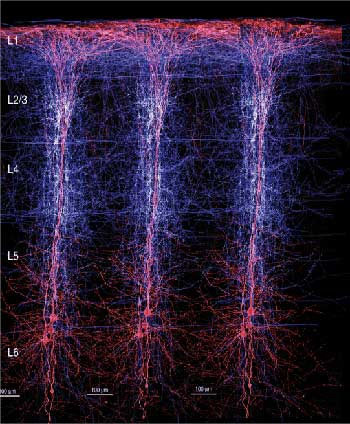
\includegraphics[width=1.0\textwidth]{images/neocortex_column.jpg}
            \end{center}

            \end{figure}

    	\end{column}
    	\begin{column}{0.7\textwidth}

            \begin{figure}[ht]

            \begin{center}
            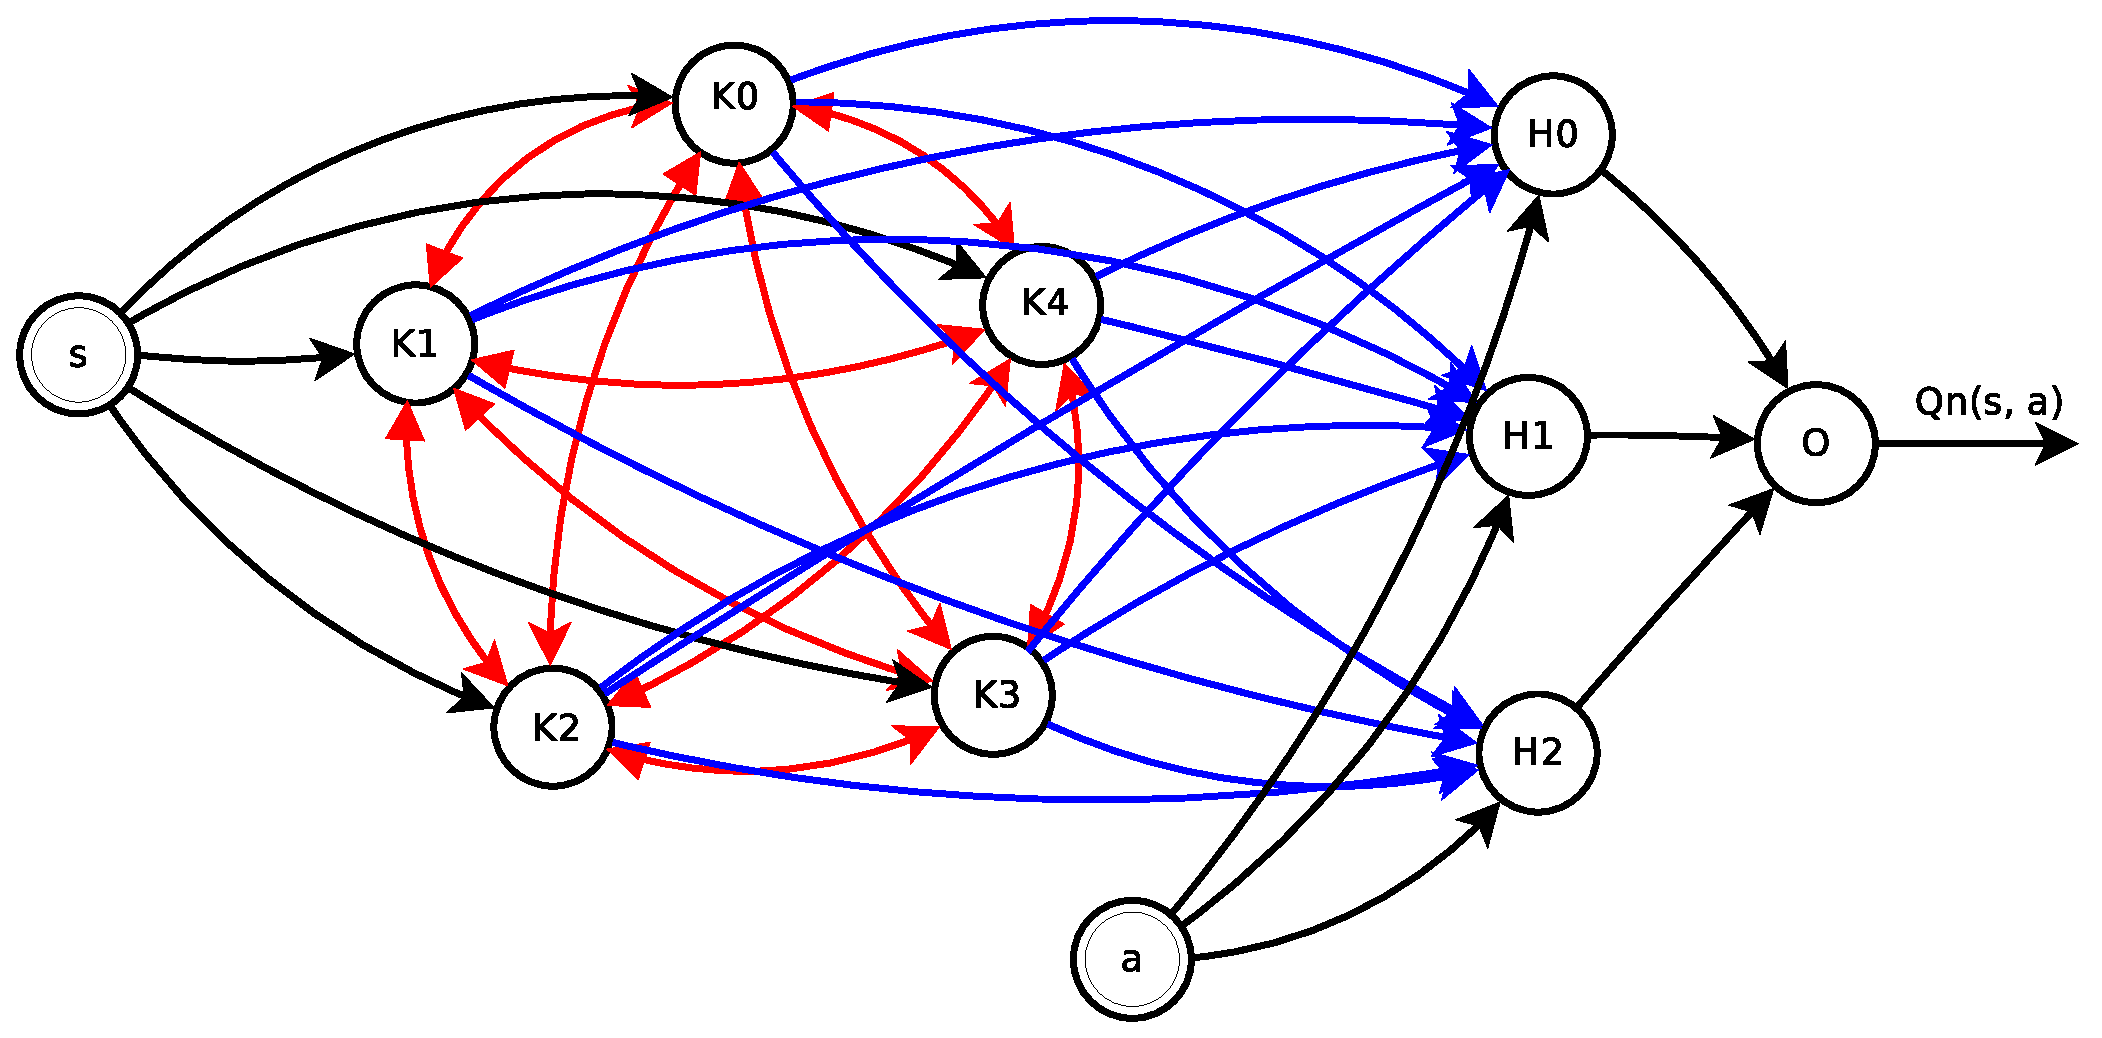
\includegraphics[width=1.0\textwidth]{block_diagram/q_learning_knn.eps}
            \end{center}

            \end{figure}

    	\end{column}
    \end{columns}

\end{frame}



%-------------------------------------------------------------------------------------
\begin{frame}[fragile]{\bf Prebiehajúci experiment - hľadanie cieľa na mape}

    \begin{columns}
    	\begin{column}{0.4\textwidth}

            \begin{figure}[ht]

            \begin{center}
            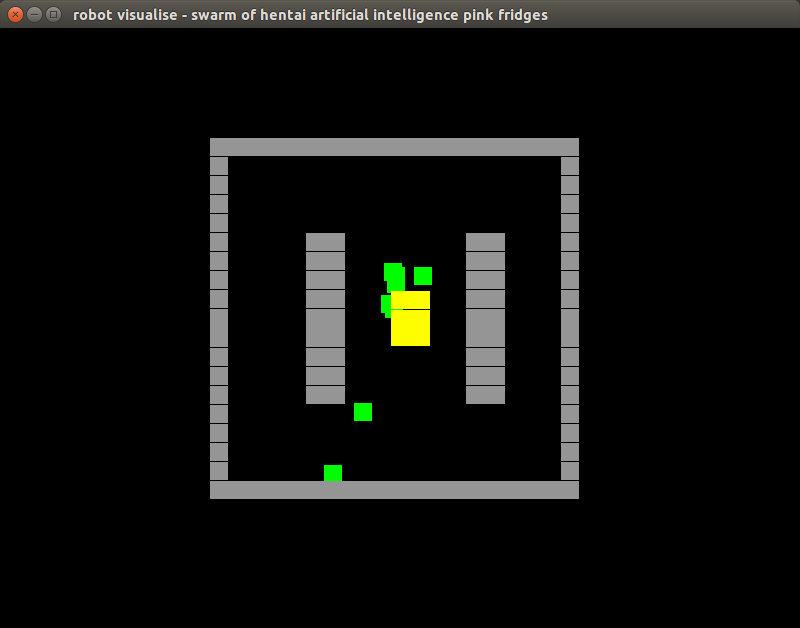
\includegraphics[width=1.0\textwidth]{images/robots.png}
            \end{center}

            \end{figure}

    	\end{column}
    	\begin{column}{0.8\textwidth}

            \begin{figure}[ht]

            \begin{center}
            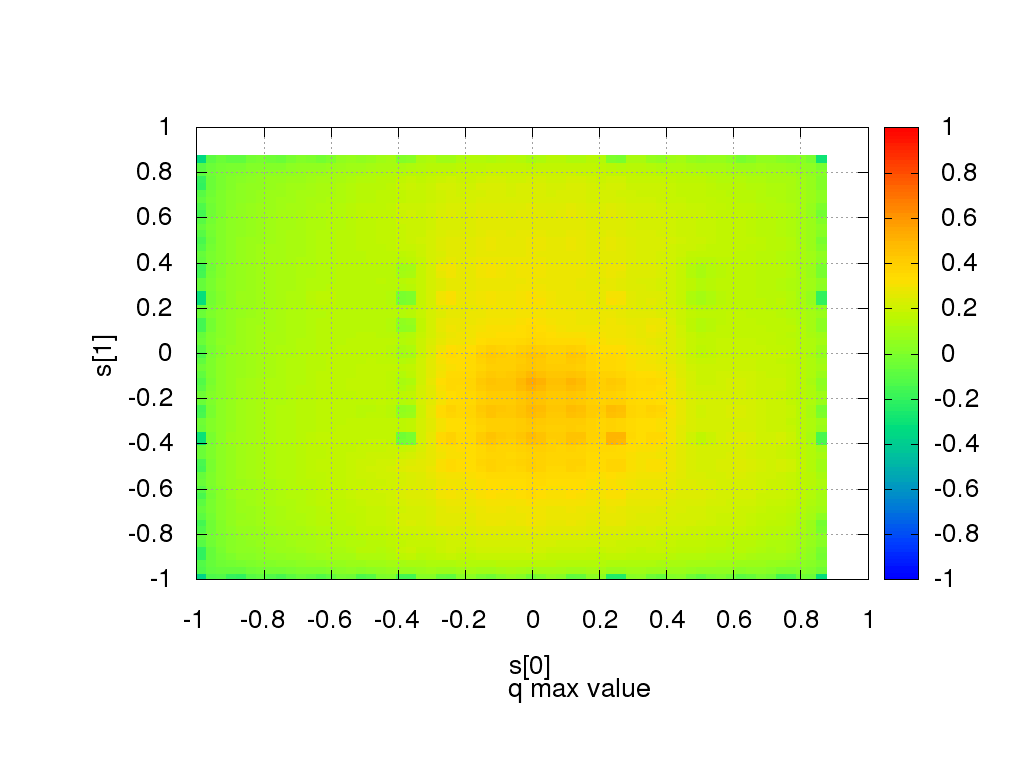
\includegraphics[width=1.0\textwidth]{images/q_max_grad.png}
            \end{center}

            \end{figure}

    	\end{column}
    \end{columns}

\end{frame}


%-------------------------------------------------------------------------------------
\begin{frame}[fragile]{\bf Prebiehajúci experiment - učiaci sa regulačný systém}

    \begin{columns}
    	\begin{column}{0.5\textwidth}

            \begin{figure}[ht]

            \begin{center}
            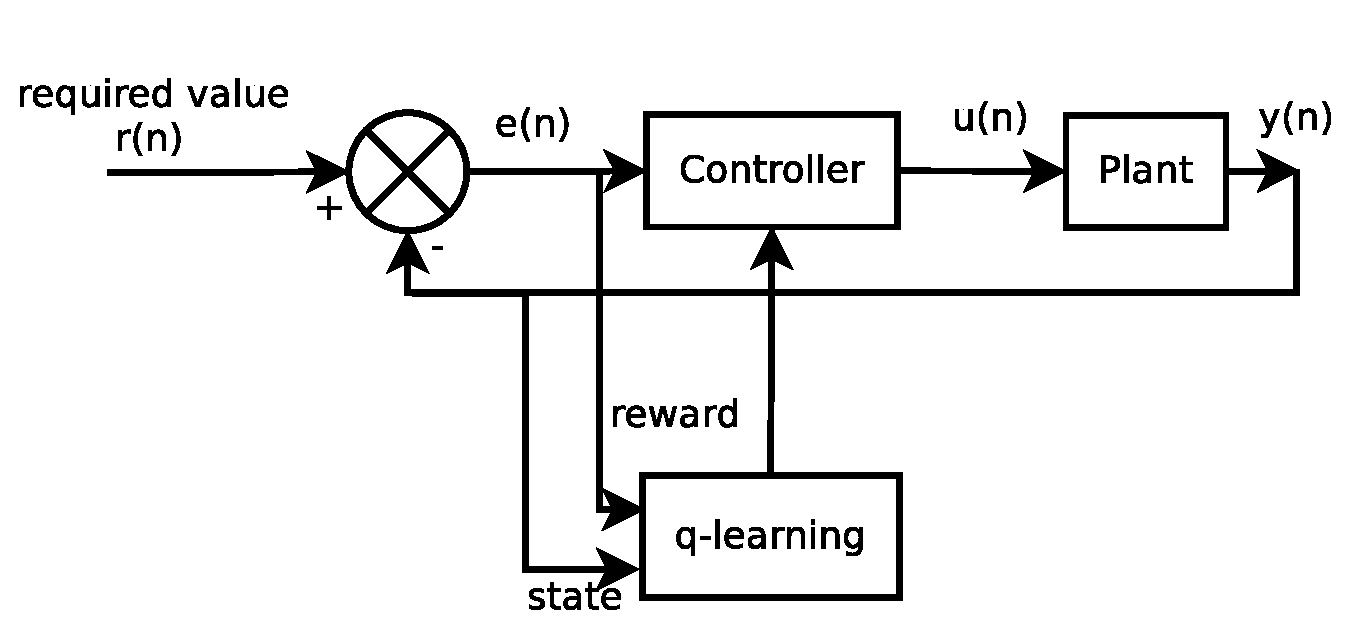
\includegraphics[width=1.0\textwidth]{diagrams/controller.eps}
            \end{center}

            \end{figure}

    	\end{column}
    	\begin{column}{0.5\textwidth}

            \begin{figure}[ht]

            \begin{center}
            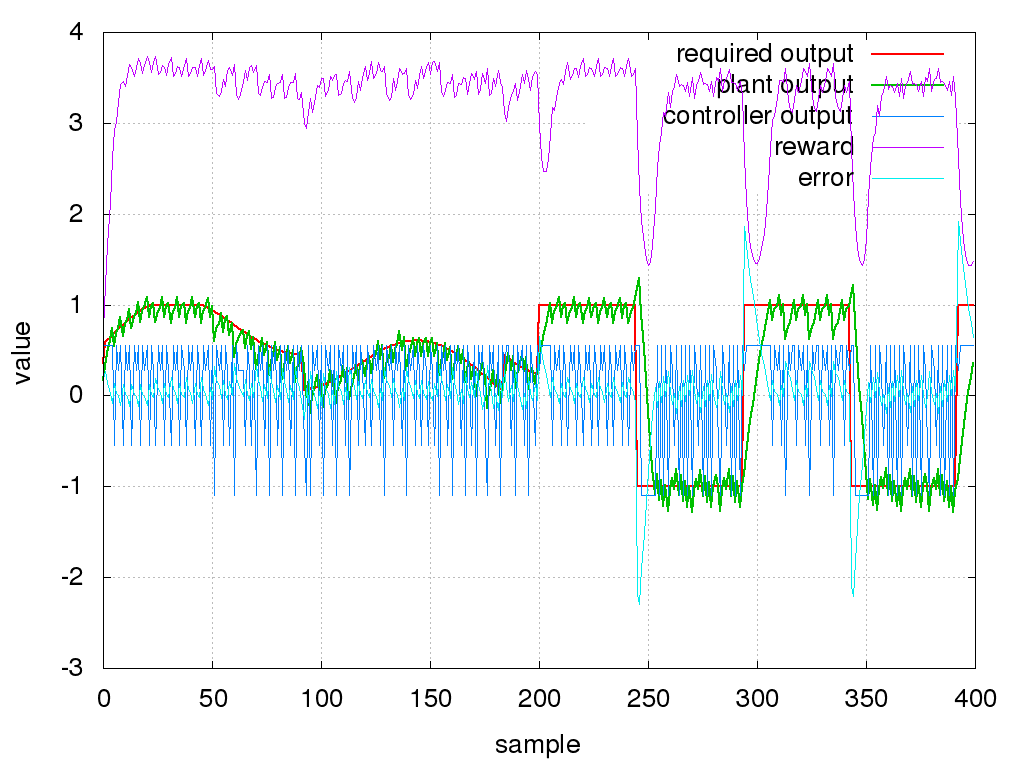
\includegraphics[width=1.0\textwidth]{images/response_log.png}
            \end{center}

            \end{figure}

    	\end{column}
    \end{columns}

\end{frame}


%-------------------------------------------------------------------------------------
\begin{frame}{\bf Ďakujem za pozornosť}

\begin{figure}[ht]
\begin{center}
\begin{minipage}{0.8\linewidth}
\begin{center}
  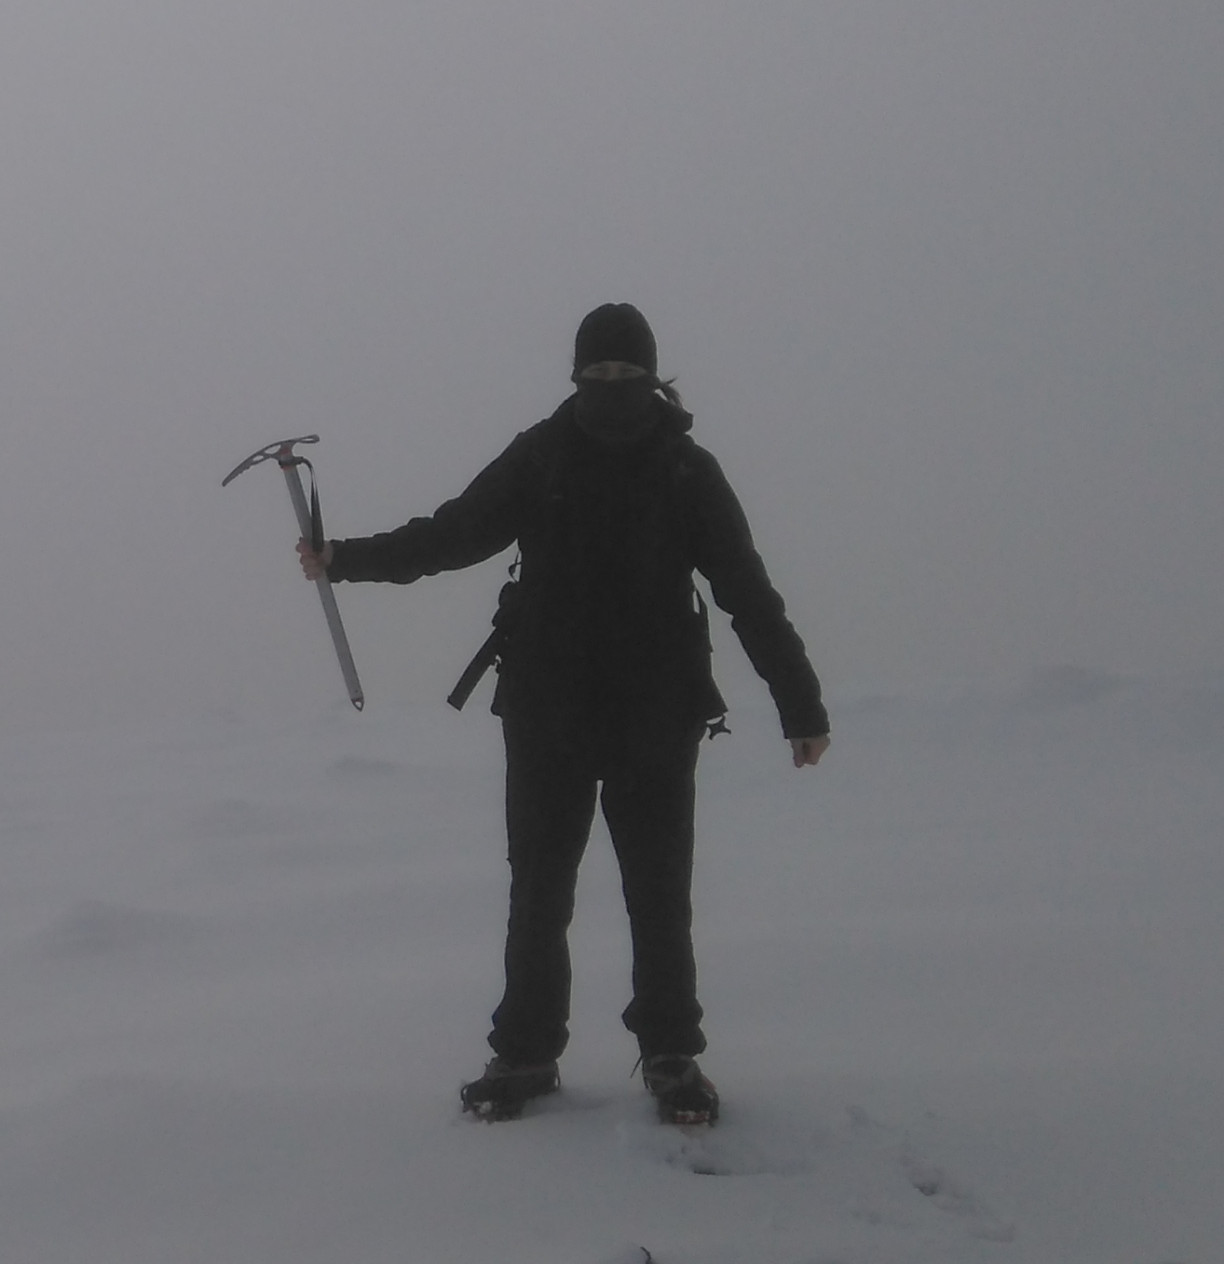
\includegraphics[width=1.0\textwidth]{images/me.jpg}
\end{center}
\end{minipage}
\end{center}
\end{figure}


\centerline{michal.chovanec@yandex.com}

\end{frame}

\end{document}
